%----------------------------------------------------------------------------------------
%	Capítulo 3
%----------------------------------------------------------------------------------------

\doublespacing
%% NUEVO CAPITULO X
\chapter{Diseño Mecatrónico}

%% NUEVA SECCIÓN X.X
\section{Desarrollo de proyecto conceptual}

El diseño conceptual es parte del proceso de diseño en la que -mediante la identificación de problemas esenciales a través de la abstracción, el establecimiento de estructuras funcionales, búsqueda de principios de funcionamiento adecuados y su combinación en una estructura global- se establece a través de la elaboración de un principio de solución.\cite[p.~159]{Pahl2007}

%% NUEVO SUBSECCION X.X.X
\subsection{Lista de requerimientos}

La lista de requerimientos (Tabla REF) se formuló mediante la realización de entrevistas (Anexo  A1) en las cuales se recopilaron aspectos requerimientos implícitos y explícitos de calidad y cantidad que debe tener el sistema en general. Dicha entrevista se planteó con las recomendaciones que muestra el libro \textit{Engineering Design}\footnote{Engineering Design – A Systematic Approach.\cite[p.~144-158]{Pahl2007}}.

\begin{savenotes}
	% Please add the following required packages to your document preamble:
	% \usepackage{multirow}
	% \usepackage[table,xcdraw]{xcolor}
	% If you use beamer only pass "xcolor=table" option, i.e. \documentclass[xcolor=table]{beamer}
	% \usepackage{longtable}
	% Note: It may be necessary to compile the document several times to get a multi-page table to line up properly
	\scriptsize
	\begin{longtable}{|c|p{0.6cm}|p{10cm}|c|}		
		\caption{Resumen de los requerimientos del sistema.}
		\label{tab:resumen de los requerimientos del sistema}\\
		\hline
		\rowcolor[HTML]{A6A6A6} 
		\multicolumn{4}{|c|}{\cellcolor[HTML]{A6A6A6}{\color[HTML]{000000} \textbf{LISTA DE REQUERIMIENTOS}}} \\ \hline
		\endfirsthead
		%
		\multicolumn{4}{c}%
		{{Tabla \thetable\ continuación de la anterior página.}} \\
		\hline
		\rowcolor[HTML]{A6A6A6} 
		\multicolumn{4}{|c|}{\cellcolor[HTML]{A6A6A6}{\color[HTML]{000000} \textbf{LISTA DE REQUERIMIENTOS}}} \\ \hline
		\rowcolor[HTML]{D9D9D9} 
		\textbf{PROYECTO} &
		\multicolumn{2}{c|}{\cellcolor[HTML]{D9D9D9}\textbf{\begin{tabular}[c]{@{}c@{}}DISEÑO DE CLASIFICADORA Y CONTADORA\\  DE TRUCHAS ARCOÍRIS (Oncorhynchus mykiss)\\ DE 10 A 20 CM. PARA LA CRIANZA DE TRUCHAS\\ EN LA LAGUNA DE PAUCARCOCHA\end{tabular}}} &
		\textbf{\begin{tabular}[c]{@{}c@{}}Fecha:\\ 2020-05-07\\ Página 1 de 1\end{tabular}} \\ \hline
		\rowcolor[HTML]{D9D9D9} 
		{\color[HTML]{000000} \textbf{\begin{tabular}[c]{@{}c@{}}Última \\ modificación\end{tabular}}} &
		{\color[HTML]{000000} \textbf{\begin{tabular}[c]{@{}c@{}}D/\\ E\end{tabular}}} &
		\multicolumn{1}{c|}{\cellcolor[HTML]{D9D9D9}{\color[HTML]{000000} \textbf{Requerimientos}}} &
		{\color[HTML]{000000} \textbf{Reponsable}} \\ \hline
		\endhead
		%
		\rowcolor[HTML]{D9D9D9} 
		\textbf{PROYECTO} &
		\multicolumn{2}{c|}{\cellcolor[HTML]{D9D9D9}\textbf{\begin{tabular}[c]{@{}c@{}}DISEÑO DE CLASIFICADORA Y CONTADORA\\  DE TRUCHAS ARCOÍRIS (Oncorhynchus mykiss)\\ DE 10 A 20 CM. PARA LA CRIANZA DE TRUCHAS\\ EN LA LAGUNA DE PAUCARCOCHA\end{tabular}}} &
		\textbf{\begin{tabular}[c]{@{}c@{}}Fecha:\\ 2020-05-07\\ Página 1 de 1\end{tabular}} \\ \hline
		\rowcolor[HTML]{D9D9D9} 
		{\color[HTML]{000000} \textbf{\begin{tabular}[c]{@{}c@{}}Última \\ modificación\end{tabular}}} &
		{\color[HTML]{000000} \textbf{\begin{tabular}[c]{@{}c@{}}D/E\footnote{Deseo (D) y exigencia (E).}\end{tabular}}} &
		\multicolumn{1}{c|}{\cellcolor[HTML]{D9D9D9}{\color[HTML]{000000} \textbf{Requerimientos}}} &
		{\color[HTML]{000000} \textbf{Reponsable}} \\ \hline
		
		
					&    & \underline{Función principal:}																										& P.D.V. 	\\
		2019-09-24  & E  & Clasificar y contar truchas arcoíris de 10 a 20 $ cm $. en al menos 2 salidas y enviar un reporte de la clasificación y el conteo.   & \multicolumn{1}{l|}{}	\\ 
					&    & \underline{Geometría:}																												& \multicolumn{1}{l|}{}	\\
		2019-09-24  & E  & El sistema no debe exceder los 200x200x200 $ cm $.																					& \multicolumn{1}{l|}{}	\\ 
					&    & \underline{Fuerzas:}																													& \multicolumn{1}{l|}{}	\\
		2019-09-24  & E  & Pesar menos de 200 $ kg $.																											& \multicolumn{1}{l|}{}	\\ 
					&    & \underline{Energía:}																													& \multicolumn{1}{l|}{}	\\
		2019-10-05  & E  & Usará baterías DC.																													& \multicolumn{1}{l|}{}	\\ 	
		2019-09-24  & E  & Funcionar desde -10 a 40 °C.																											& \multicolumn{1}{l|}{}	\\ 	
		2019-09-24  & D  & La máquina debe enviar la información.																								& \multicolumn{1}{l|}{}	\\ 	
					&    & \underline{Materiales:}																												& \multicolumn{1}{l|}{}	\\
		2019-09-22  & E  & La máquina debe ser inoxidable.																										& \multicolumn{1}{l|}{}	\\ 	
		2019-09-20  & E  & La máquina no debe desprender ningún residuo que pueda contaminar el agua.															& \multicolumn{1}{l|}{}	\\ 	
		2019-09-25  & D  & Los materiales de manufactura deben poder ser adquiridos en el mercado peruano.														& \multicolumn{1}{l|}{}	\\ 			
					&    & \underline{Señales:}																													& \multicolumn{1}{l|}{}	\\
		2019-09-24  & E  & Se debe enviar una señal en caso de fallo del sistema y pausar el proceso.															& \multicolumn{1}{l|}{}	\\ 	
					&    & \underline{Hardware:}																												& \multicolumn{1}{l|}{}	\\
		2019-10-05  & E  & La máquina debe usar cámaras o dispositivos similares para obtener imágenes.															& \multicolumn{1}{l|}{}	\\ 		
					&    & \underline{Software:}																												& \multicolumn{1}{l|}{}	\\
		2019-10-05  & D  & El sistema generará un reporte de la clasificación y conteo.																			& \multicolumn{1}{l|}{}	\\ 	
					&    & \underline{Costos:}   																												& \multicolumn{1}{l|}{}	\\ 
		2019-09-24  & D  & El precio unitario menor a 10 mil dólares.       								    												& \multicolumn{1}{l|}{}	\\  \hline
		
		
		\rowcolor[HTML]{D9D9D9} 
		\multicolumn{1}{|l|}{\cellcolor[HTML]{D9D9D9}{\color[HTML]{000000} }} &
		\multicolumn{2}{c|}{\cellcolor[HTML]{D9D9D9}{\color[HTML]{000000} \textbf{Última modificación: 2019-10-05}}} &
		{\color[HTML]{000000} } \\ \hline
	\end{longtable}

\end{savenotes}

%% NUEVO SUBSECCION X.X.X
\subsection{Caja negra}

La caja negra mostrada en la Figura \ref{fig:caja negra del sistema} representa la energía (flecha continua), materia (flecha gruesa) y señales (flecha discontinua) que necesita y brinda el sistema para funcionar como un sistema clasificador y contador de truchas de un determinado rango según la lista de requerimientos mostrada en la Tabla REF.

\begin{figure}[H]
	\centering
	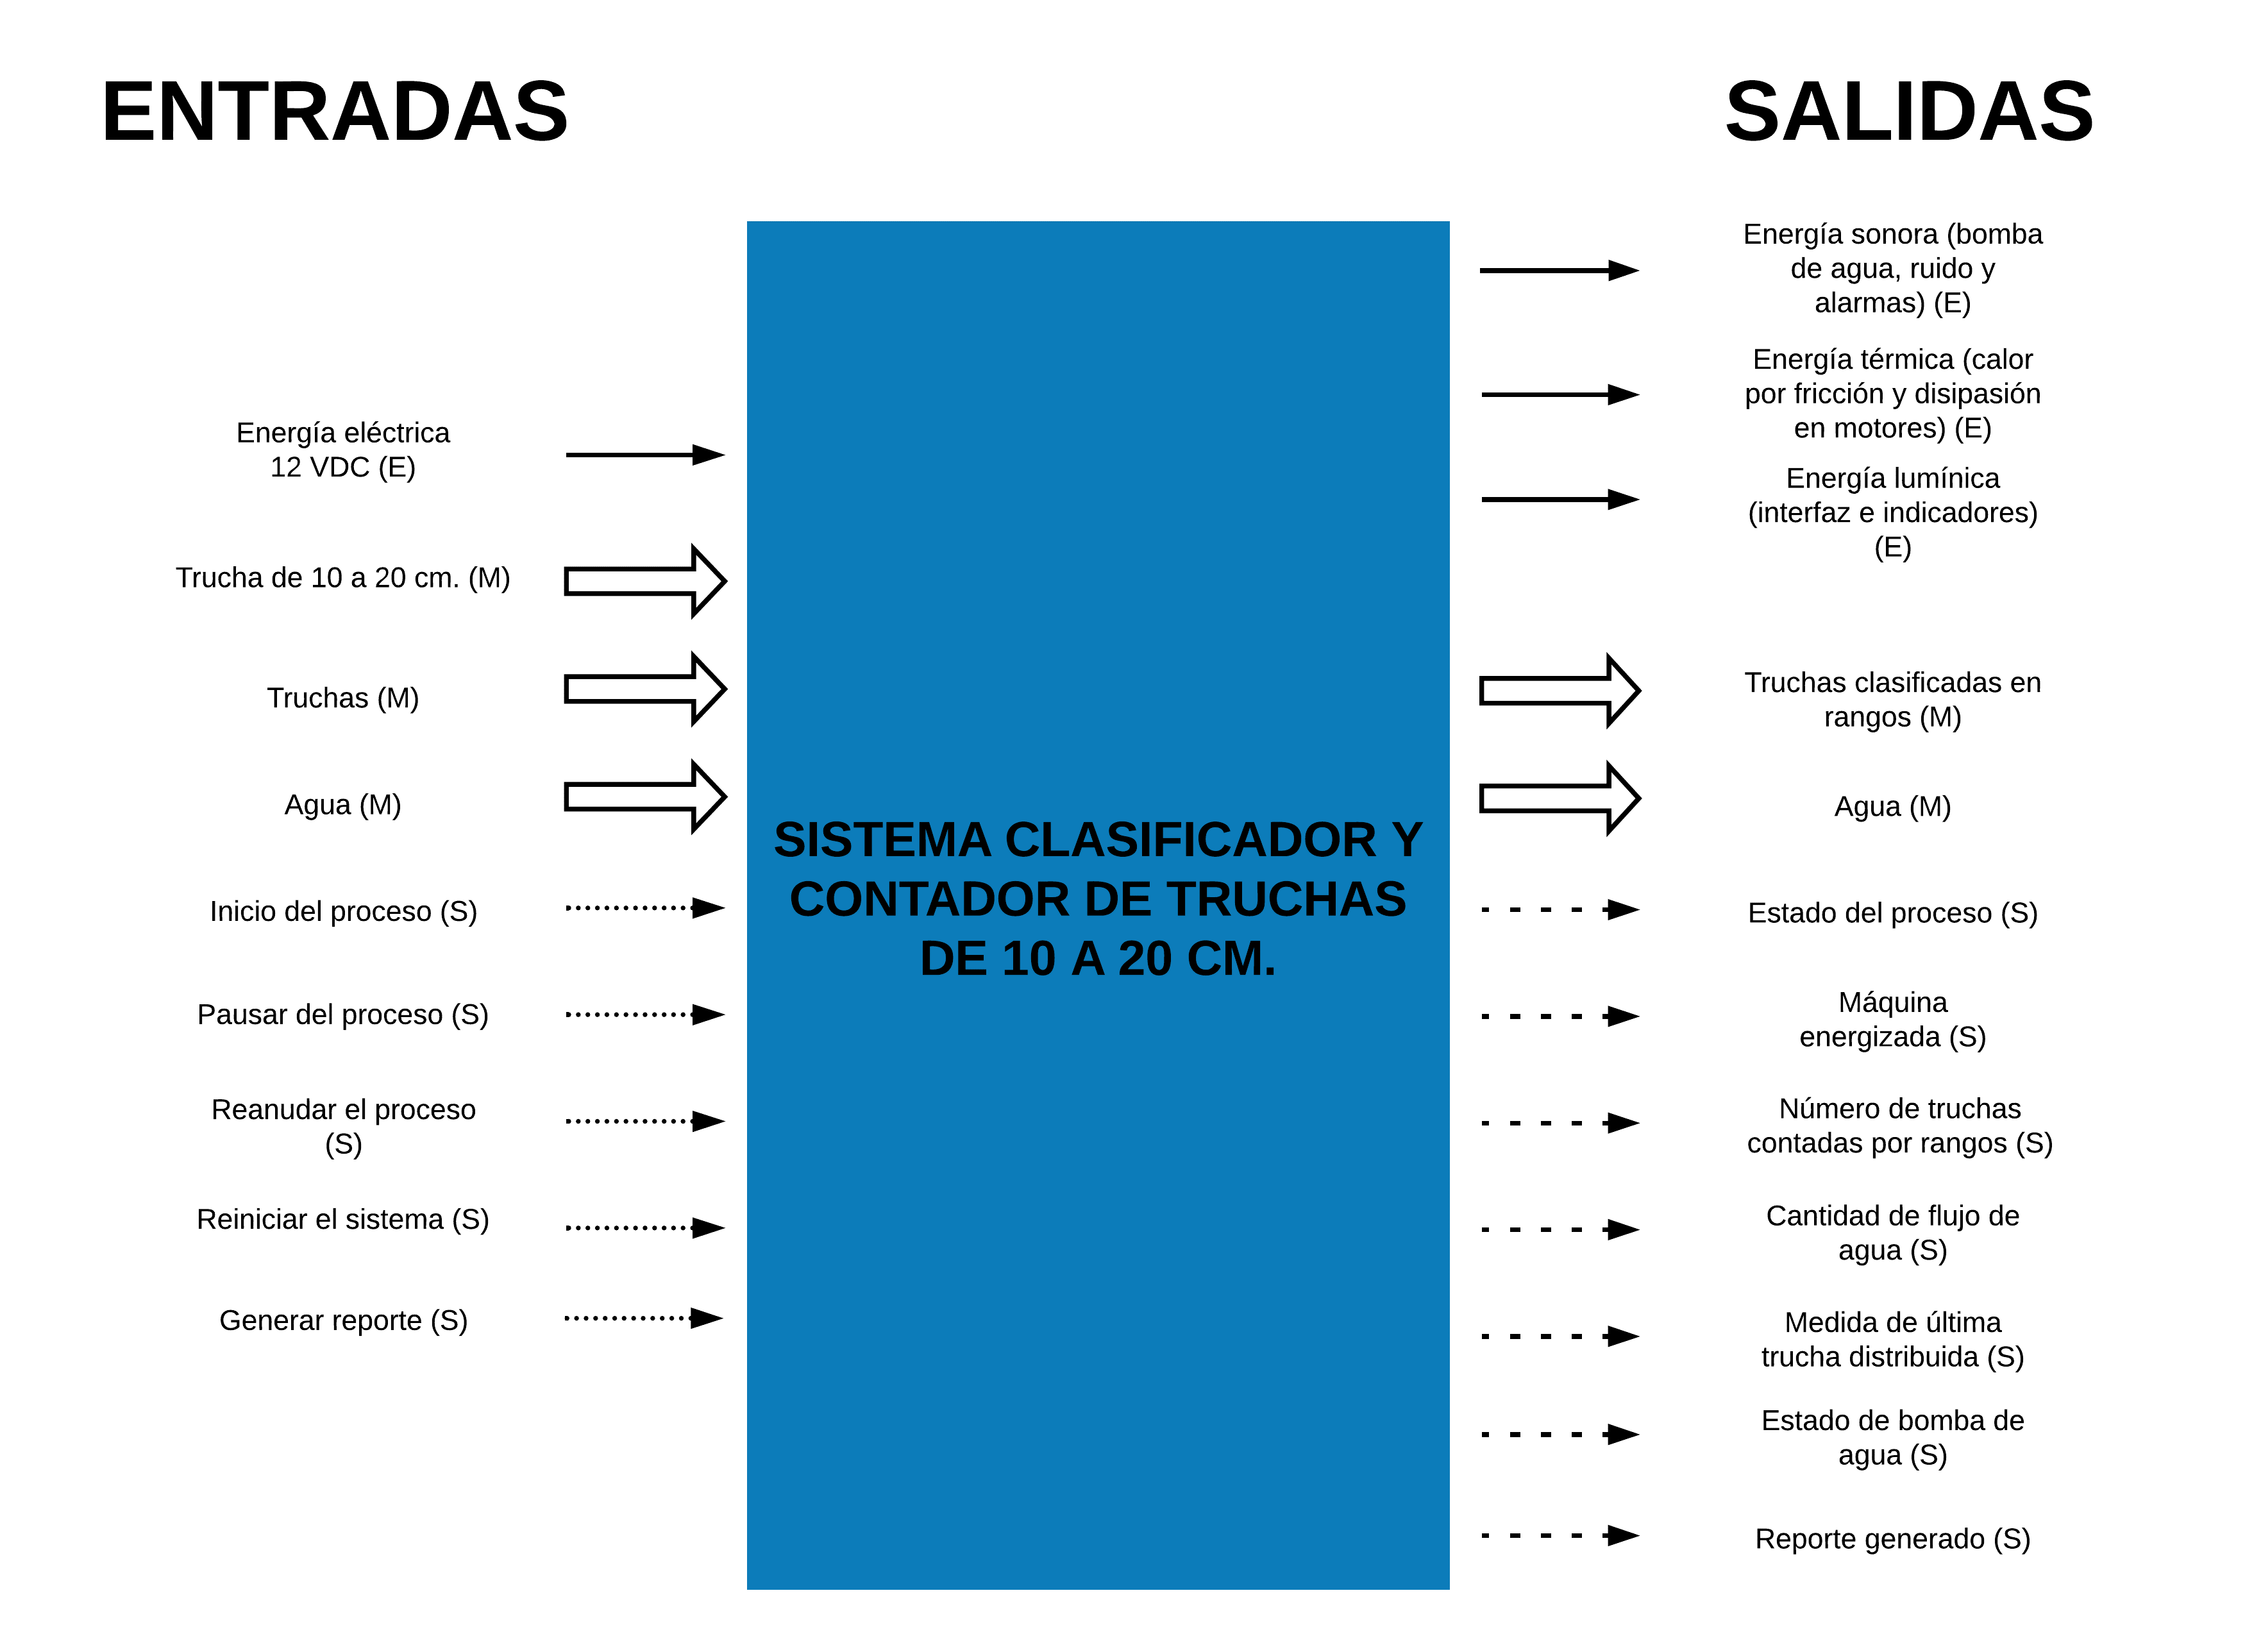
\includegraphics[width=1\textwidth]{chapter3/caja negra del sistema.png}
	\caption{Caja negra del sistema.}
	Fuente: Elaboración propia.
	\label{fig:caja negra del sistema}
\end{figure}

%% NUEVA SUB-SUB-SECCION X.X.X.X
\subsubsection{Función principal}

El sistema tiene como función principal clasificar truchas que provienen de un estanque o jaula flotante que tiene truchas que necesitan ser redistribuidas según sus dimensiones.

%% NUEVA SUB-SUB-SECCION X.X.X.X
\subsubsection{Entradas}

El sistema tiene entradas de diversos tipos: energía, materia y señal. La entrada de energía es únicamente una batería de 12 VDC ya que es portable; Las entradas de materia son indispensablemente el agua y las truchas a clasificar; Las señales de entrada para este proceso son las básicas para cualquier proceso de este tipo (\textit{iniciar, pausar, reanudar y reiniciar}), además la señal de generar un reporte para ser analizado y mantener control sobre el cultivo.

%% NUEVA SUB-SUB-SECCION X.X.X.X
\subsubsection{Salidas}

De manera similar a las entradas, las salidas se dividen en energía, materia y señal: El sistema genera tres tipos de energía debido a los actuadores, ruido, alarmas, interfaz e indicadores; Las truchas divididas en hasta tres rangos salen de manera separada; Se muestra el estado del proceso, estado del sistema, número de truchas contadas dependiendo del rango, medida de la última trucha distribuida, estado de la bomba de agua y la señal de reporte generado.

%% NUEVO SUBSECCION X.X.X
\subsection{Estructura de funciones}

Una vez que se ha formulado la caja negra es posible indicar, con el uso de diagrama de bloques, expresar la relación entre entradas y salidas con una solución neutral. Esta relación debe tener la mayor precisión posible. La estructura de funciones global puede desglosarse en sistemas que a su vez se subdividen en funciones.\cite[p.~169-181]{Pahl2007}

\newpage
\thispagestyle{mylandscape}
\begin{landscape}
	\begin{figure}[H]
		\centering
		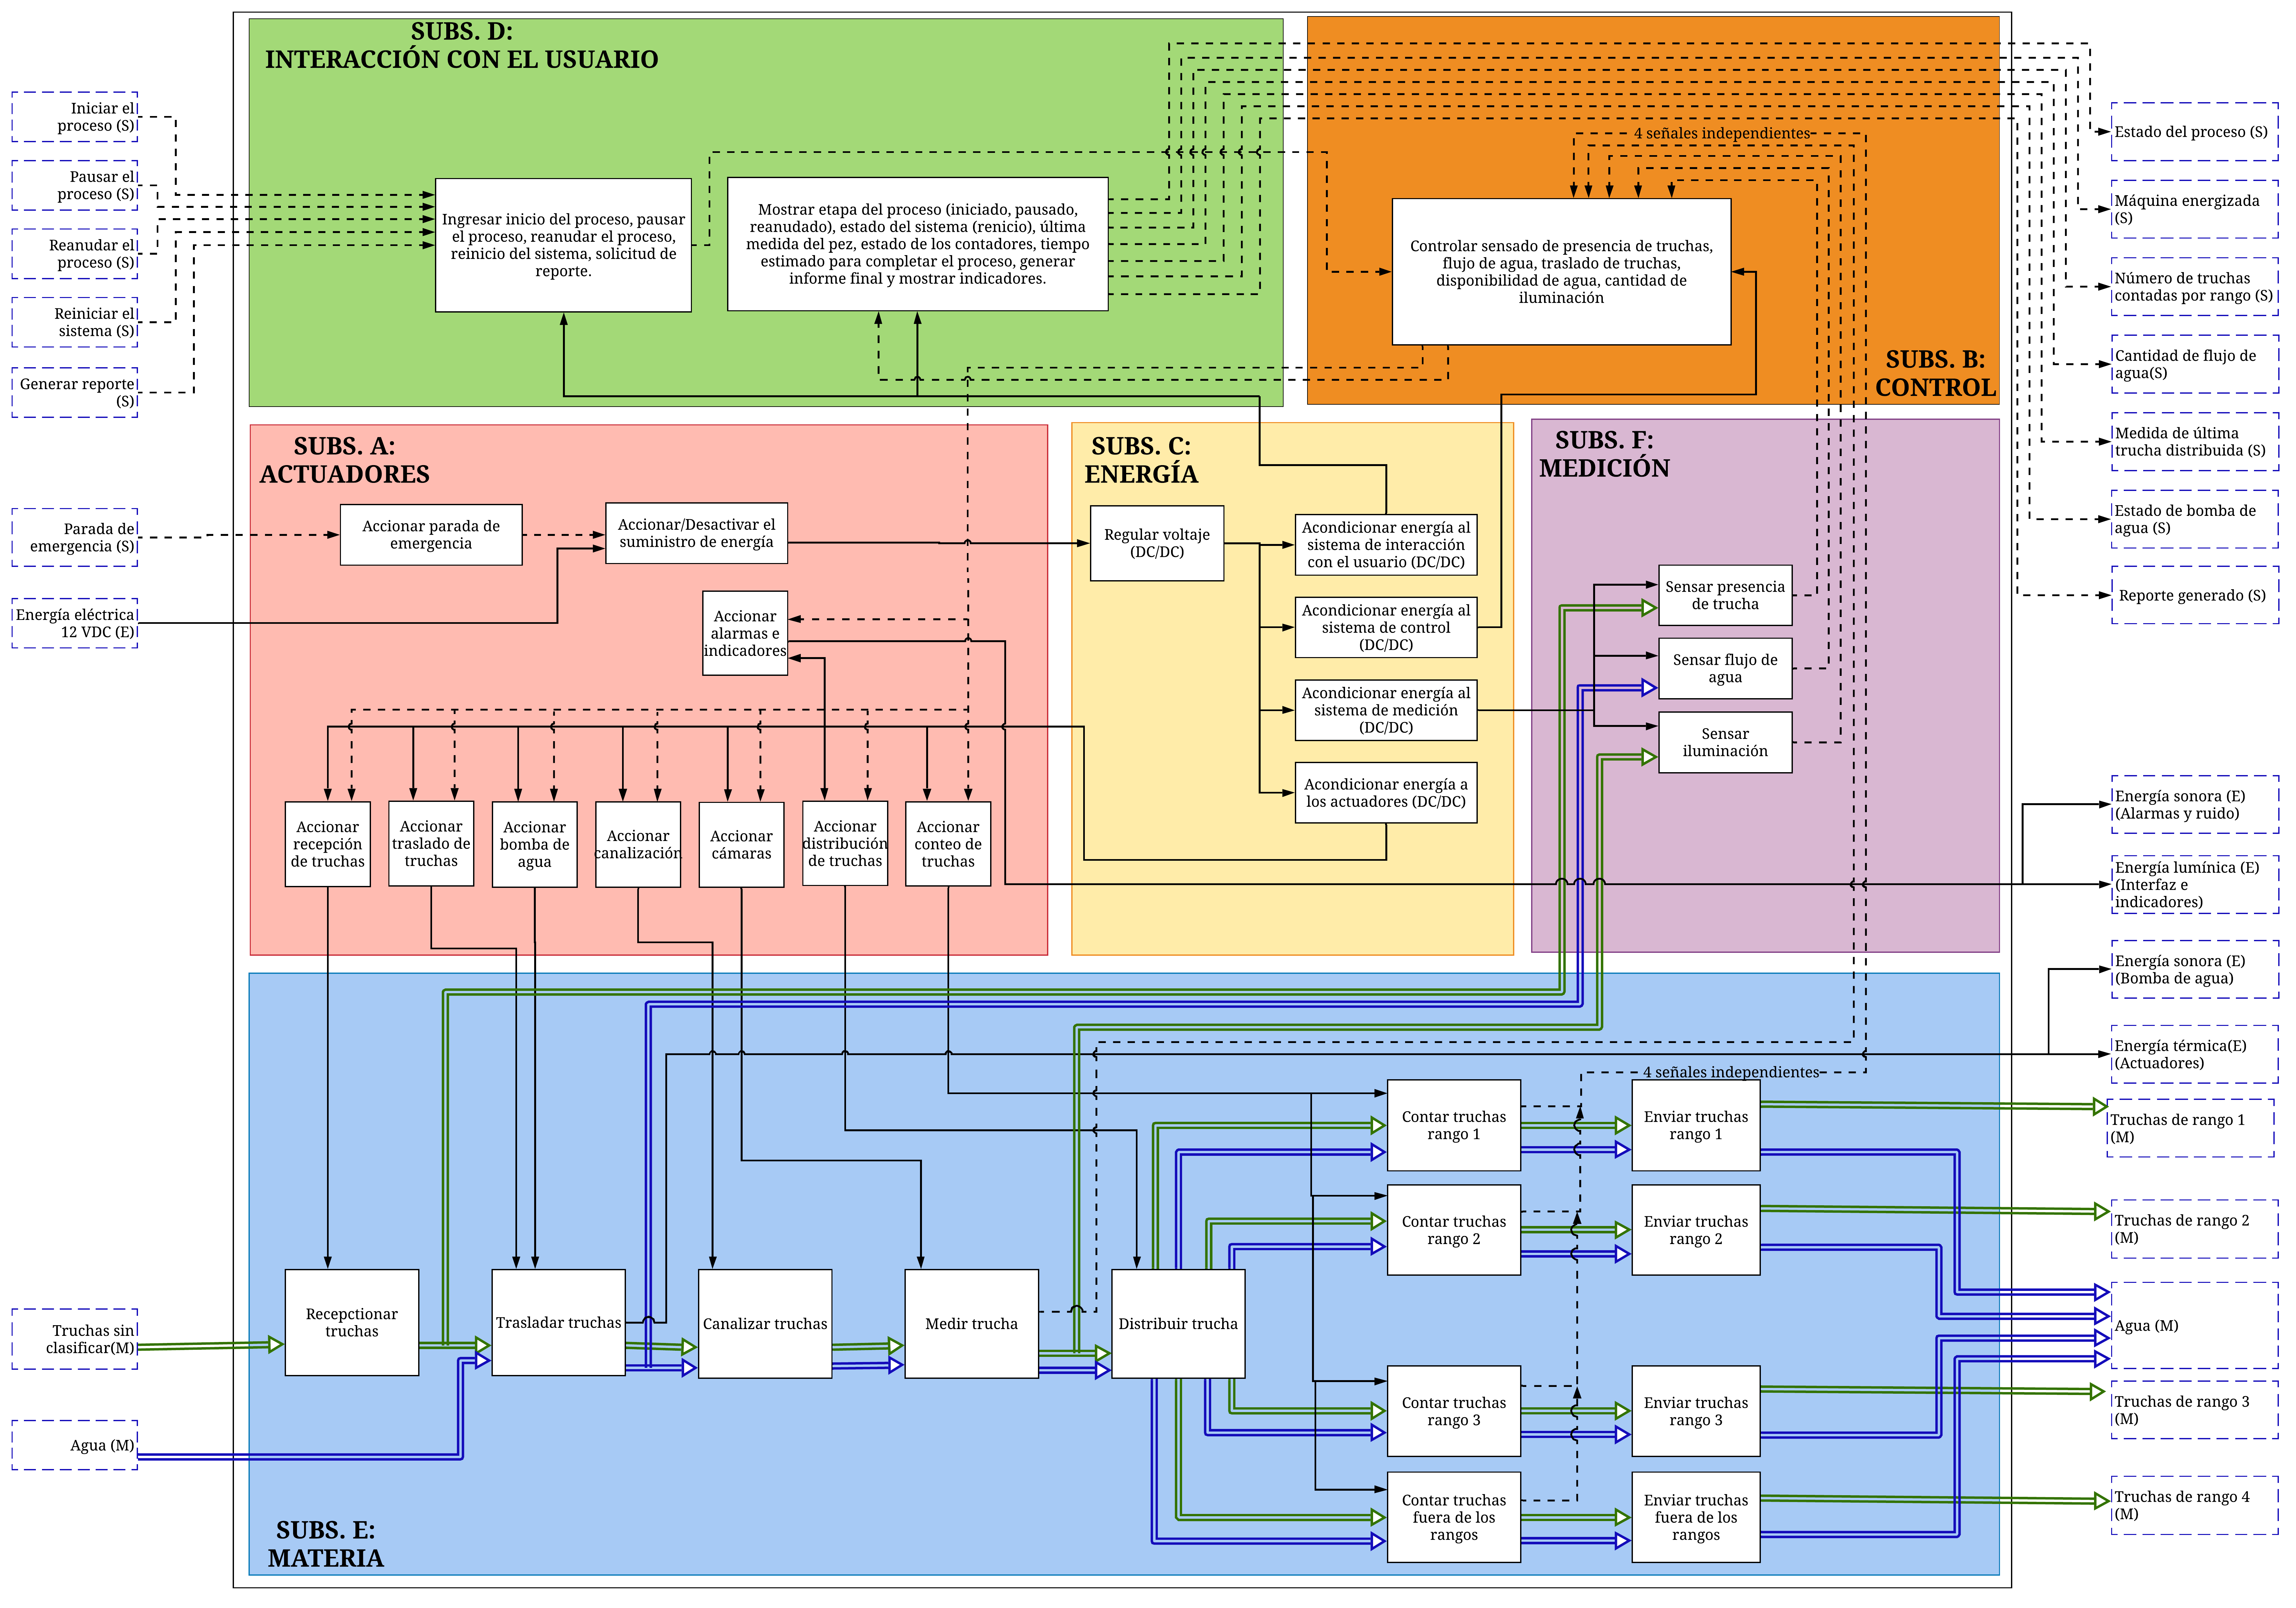
\includegraphics[width=0.95\paperwidth]{chapter3/estructura global de funciones.png}
		\caption{Estructura global de funciones.}
		Fuente: Elaboración propia.
		\label{fig:estructura global de funciones}
	\end{figure}
\end{landscape}

\newpage
\thispagestyle{fancy}
%% NUEVA SUB-SUB-SECCION X.X.X.X
\subsubsection{Lista de funciones por subsistema}

El sistema propuesto consta de seis subsistemas: actuadores, control, energía, interacción con el usuario, materia y medición. El propósito y funciones de cada subsistema se indica en las siguientes líneas.

\begin{enumerate}
	
	\item \textbf{Subsistema A: Actuadores}\\ El subsistema integra el accionamiento de los mecanismos que transforman que permiten distribuir la materia en los rangos requeridos.
		
		\begin{enumerate}[label=\Alph*)] % \alph for lowercase
			\item	\textbf{Accionar parada de emergencia:} Esta función permite conectar o desconectar físicamente la energía de entrada del resto del sistema.
			
			\item	\textbf{Accionar/Desactivar el suministro de energía:} Esta función se encargará de proveer energía al sistema para dar inicio al proceso al momento que recibe la señal de inicio.
			
			\item	\textbf{Accionar recepción de truchas:}
			Esta función activa o desactiva la entrada de materia al sistema, en este ca-so el ingreso de truchas al sistema.
			
			\item	\textbf{Accionar traslado de truchas:}
			Esta función activa o desactiva la función que recibe truchas y agua para poder desplazar a las truchas dentro del sistema.
			
			\item	\textbf{Accionar bomba de agua:}
			Esta función activa, desactiva y regula el flujo de agua dentro del sistema. 
			
			\item	\textbf{Accionar canalización:}
			Esta función activa o desactiva el sistema de canalización del sistema, es decir, controla la función que regula el paso de una sola trucha por vez a las si-guientes partes del sistema.
			
			\item	\textbf{Accionar cámaras:}
			Esta función activa, desactiva y prepara la adquisición de imágenes o vi-deo del sistema.
			
			\item	\textbf{Accionar distribución de truchas:}
			Esta función se encarga de la distribución de las truchas según su rango dentro del sistema.
			
			\item	\textbf{Accionar alarmas e indicadores:}
			Acciona las alarmas e indicadores del sistema para poder informar al ope-rario de la situación del proceso.
			
		\end{enumerate}
	
	\item \textbf{Subsistema B: Control}\\ El subsistema de control garantiza la precisión de los mecanismos, la calidad de los procesos, la seguridad del sistema.
		\begin{enumerate}[label=\Alph*)] % \alph for lowercase
			\item \textbf{Función general:} Esta función controla el sensado de presencia de trucha, flujo de agua, traslado de truchas, sensado de disponibilidad de agua y cantidad de iluminación.			
		\end{enumerate}
	
	\item \textbf{Subsistema C: Energía}\\ El subsistema de energía mantiene el funcionamiento continuo del sistema para reali-zar sus funciones características a través de una fuente de energía. 
	
	\begin{enumerate}[label=\Alph*)] % \alph for lowercase
		\item	\textbf{Regular voltaje ($ DC/DC $):}		Esta función acondiciona la energía de entrada (12 VDC) a la energía necesaria para el sistema.
		
		\item	\textbf{Acondicionar energía al sistema de interacción con el usuario ($ DC/DC $):}		Esta función acondiciona la energía de entrada (12 VDC) a la energía necesaria para el sistema de interacción con el usuario.
		
		\item	\textbf{Acondicionar energía al sistema de control ($ DC/DC $):}	Esta función acondiciona la energía de entrada (12 VDC) a la energía necesaria para el sistema de control
		
		\item	\textbf{Acondicionar energía al sistema de medición ($ DC/DC $):}	Esta función acondiciona la energía de entrada (12 VDC) a la energía necesaria para el sistema de medición.
		
		\item	\textbf{Acondicionar energía a los actuadores ($ DC/DC $):} Esta función acondiciona la energía de entrada (12 VDC) a la energía necesaria para el sistema de los actuadores.
		
	\end{enumerate}
	
	\item \textbf{Subsistema D: Interacción con el usuario}\\ Este subsistema permite la comunicación entre el usuario final / operador y el sistema. Facilita la realización del proceso completo, permitiendo al usuario contar con información importante del proceso para poder tomar decisiones de forma rápida.
	
	\begin{enumerate}[label=\Alph*)] % \alph for lowercase
		\item	\textbf{Función ingreso de señales:}		Esta función recibe las señales de entrada como inicio, pausar, reanudar y reiniciar el proceso. Además, recibe la solicitud de reporte. Usa esta información y la envía al subsistema de control.
		
		\item	\textbf{Función mostrar señales:}		Esta función muestra las etapas del proceso (iniciar, pausar, reanudar y reiniciar). También muestra la medida de la última trucha que se distribuyó, estado de los contadores, tiempo estimado para completar el proceso, informe generado y mostrar indicadores.
		
	\end{enumerate}

	\item \textbf{Subsistema E: Materia}\\ El subsistema de materia contiene las funciones que se encargan de distribuir la mate-ria en rangos que se ingresan al sistema. Las funciones se desarrollan como una secuencia de tareas.

	\begin{enumerate}[label=\Alph*)] % \alph for lowercase
		\item	\textbf{Recepcionar truchas:}
		Esta función mediante mecanismos recibe indicaciones de otras partes del sistema para accionarse. Es el primer módulo que recepciona a las truchas. 
		
		\item	\textbf{Trasladar truchas:}
		Este mecanismo recibe agua y a las truchas que salen de la función “recepcionar truchas”. Impulsa mediante un flujo de agua constante a las truchas a lo lar-go del sistema hasta llegar a las salidas.
		
		\item	\textbf{Canalizar truchas:}
		Este mecanismo recibe agua y truchas del módulo “trasladar truchas”. Además, es accionado por actuadores para cumplir con dejar pasar una trucha por vez al siguiente módulo del sistema.
		
		\item	\textbf{Medir trucha:}
		Este mecanismo recibe agua y truchas canalizadas del módulo anterior “canalizar truchas”. Acciona cámaras para poder realizar la toma de dimensiones de la trucha e indica al sistema el rango al que fue asignado. Este módulo clasifica virtualmente a las truchas.
		
		\item	\textbf{Distribuir trucha:}
		Este mecanismo recibe agua y trucha medida del módulo anterior “medir trucha". Es accionada y permite seleccionar según los rangos el próximo módulo correspondiente. Este módulo es el encargado de clasificar físicamente a la trucha.
		
		\item	\textbf{Contar truchas por rangos:}
		Este mecanismo recibe agua y truchas asignadas a su rango del módulo anterior “distribuir truchas”. Accionada envía señales al sistema de control sobre la cantidad de peces contados por rangos.
		
		\item	\textbf{Enviar truchas por rangos:}
		Este mecanismo permite trasladar a la trucha que ya fue contada y clasificada por el sistema por los módulos anteriores al respectivo estanque o jaula flotante asignado.
		
	\end{enumerate}
	
	
	\item \textbf{Subsistema F: Medición}\\ El subsistema de medición se encarga de sensar las variables del proceso necesarias para ejercer un óptimo control del sistema y minimizar el error. Se considera las siguientes funciones como esenciales.

	\begin{enumerate}[label=\Alph*)] % \alph for lowercase
		\item	\textbf{Sensar presencia de trucha:}
		Esta función detecta si las truchas han ingresado al sistema o siguen dentro del sistema.
		
		\item	\textbf{Sensar flujo de agua:}
		Esta función mide el flujo de agua dentro del sistema para mantenerlo constante para reducir el estrés hídrico.
		
		\item	\textbf{Sensar iluminación:}
		Esta función sensa la iluminación que es necesaria para capturar imágenes con normalidad.
		
	\end{enumerate}	
	
	
	
	%	To create new enumerate alpha use code below
	%	\begin{enumerate}[label=\Alph*)] % \alph for lowercase
	%	\end{enumerate}
\end{enumerate}
%% NUEVO SUBSECCION X.X.X
\subsection{Matriz morfológica}

%% NUEVO SUBSECCION X.X.X
\subsection{Conceptos de solución}

%% NUEVA SUB-SUB-SECCION X.X.X.X
\subsubsection{Concepto de solución N° 1}

%% NUEVA SUB-SUB-SECCION X.X.X.X
\subsubsection{Concepto de solución N° 2}

%% NUEVA SUB-SUB-SECCION X.X.X.X
\subsubsection{Concepto de solución N° 3}

%% NUEVO SUBSECCION X.X.X
\subsection{Evaluación técnico-económica}

%% NUEVA SUB-SUB-SECCION X.X.X.X
\subsubsection{Criterios técnicos}

%% NUEVA SUB-SUB-SECCION X.X.X.X
\subsubsection{Criterios económicos}

%% NUEVA SUB-SUB-SECCION X.X.X.X
\subsubsection{Elección de concepto óptimo}

%% NUEVO SUBSECCION X.X.X
\subsection{Diagrama de operaciones de solución escogida}

%%%%%%% FALTA PUNTOS 
%%%%%%% FALTA PUNTOS 
%%%%%%% FALTA PUNTOS 
%%%%%%% FALTA PUNTOS 
%%%%%%% FALTA PUNTOS 
%%%%%%% FALTA PUNTOS 
%%%%%%% FALTA PUNTOS 
%%%%%%% FALTA PUNTOS 



